%%%%%%%%%%%%%%%%%%%%%%%%%%%%%%%%%%%%%%%%%%%%%%%%%%%%%%%%%%
\section{Using Biases}
%%%%%%%%%%%%%%%%%%%%%%%%%%%%%%%%%%%%%%%%%%%%%%%%%%%%%%%%%%

This section make use of an improved central bias model (similar to \cite{clarke-tatler2014} except uses a truncated Gaussian distribution to take the image boundaries into account: see Section \ref{sec:truncatedCentral}) and the \textit{saccadic flow} model (described in Section \ref{ModellingFlow}). We present three examples of how these bias models can be used as a prior in order to weight fixations. First of all, we will demonstrate how we can weight fixations in hotspot maps to reduce the noise and give an improved visualisation of the regions of the image that participants looked at more than expect. Secondly, we will re-analyse the effect of attention on object naming from \cite{clarke2013}.  Finally, we will demonstrate how these priors can be used in ROC analysis to improve results. We will re-analyse the effect of the scene context model developed by  \cite{ehinger2009} as an example. 

\subsection{Gaze landscapes}

One technique that is commonly used to visualise the spatial allocation of gaze is to create 'heatmap' plots where colour or luminance are used to indicate the density of fixation on those locations (Figure ~\ref{fig:adjustedHeatmaps}, column 2). Some argue that one problem with visualising data in this way is that they represent all fixations as equal. For example, a fixated location with a fixation of a second would be weighted equally with fixations that lasted half that time. If we want to make an assumption that fixation duration is intimately linked with the importance of that fixation (i.e. we will look longer at more informative information) then we can change our visualisation to weight fixations by their duration (Figure ~\ref{fig:adjustedHeatmaps}, column 3).

One advantage of the \citep{clarke-tatler2014} model, and the saccadic flow model here is that we can represent fixations by the likelihood that they would occur based on the predictions of the models. As there is an image independent tendency to fixate in the centre of the scene (for example), then we might consider that saccades to locations less predicted by these behavioural and oculomotor biases might involve more high-level mechanisms. In Figure ~\ref{fig:adjustedHeatmaps} (column 4 and 5) we present some overlaid heatmap data from the \citep{clarke2013} dataset, where fixations are weighted by the inverse probability of them occurring based on the models of central bias and saccadic flow. These figures reveal that representing data in this manner can allow us to visualise information that was important enough to break the biases of looking at the scene centre, or making saccades in line with our saccadic flow model. We can therefore use this to remove some of the image-independent biases, and reveal the more important image \emph{dependent} information.

[this is all a bit rubbish - I will rewrite this but I am just quickly putting it in to remind me why I picked these images]

The top row of Figure ~\ref{fig:adjustedHeatmaps} demonstrates that weighting the fixations by the central bias and flow model both reduce the \emph{importance} of some fixations. The central bias model punishes fixations near the center of the image, while the flow model punishes fixations that were well predicted by the oculomotor biases of the saccadic flow model. Conversely, the models reward unlikely fixations. The second row reveals an instance of where the car to the left received less fixations than the pub sign, but that these fixations are boosted in the central bias and saccadic flow models where 'unlikely' saccades were made to this location. In the third and fourth rows, there are examples of images with a photographer bias of content towards the centre of the photograph. This reveals an example of where down-weighting the central fixations might lose important content.
where the central bias model reduces the influence fixations in the centre of pictures that have important content located there. Given the tendency for photographers to bias their photographs in the centre, reducing fixations to the castle in the painting (row 3) and the girl's face (row 4).

\begin{figure*}[htb]
\centering
\includegraphics[width=\textwidth]{figs/heatmap_figure.pdf}
\caption{Examples of fixation heatmap plots from \citep{clarke2013}. The same fixations are presented where the Gaussian at each fixation is weighted by the duration of the fixation, the centre bias model from \citep{clarke-tatler2014} , and the saccadic flow model presented in this paper. 
\label{fig:adjustedHeatmaps}
\end{figure*}



%\begin{figure*}
%\includegraphics[width=\textwidth]{figs/adjustedheatmaps.pdf}
%\caption{Traditional 'heat map' plots of fixations normalised by the central bias. This method allows us to characterise fixations that are less accountable for by image-independent central biases.}
%\label{fig:adjustedHeatmaps}
%\end{figure*}

Or do we call them hotspot maps?

\subsection{Reanalysis of Clarke et al 2013}
\label{sec:reanalysisClarke2013}
Do the flow-weights offer an improvement on predicting named objects over the fixations-weights?

\subsection{Reanalysis of Ehinger et al 2009}

Re-analysis of \cite{ehinger2009} comparing ROC methods for leave-one-out, uniform, central bias and flow. How well does their context model work in each test>

\subsection{Comparison between synthetic and real data}
\label{sec:humanComp}
To what extent does saccadic flow account for coarse-to-fine dynamics? Not that well. Not unexpected.

We can see from Figure \ref{fig:flowHumanComp} that both the central bias and the saccadic flow model do an good job of capturing the distribution of fixation locations in the $x$ and $y$ axes. However, the saccades generated by the flow model tend to be slightly larger than those made by human observers. 

\begin{figure*}[htb]
\centering
\subfigure{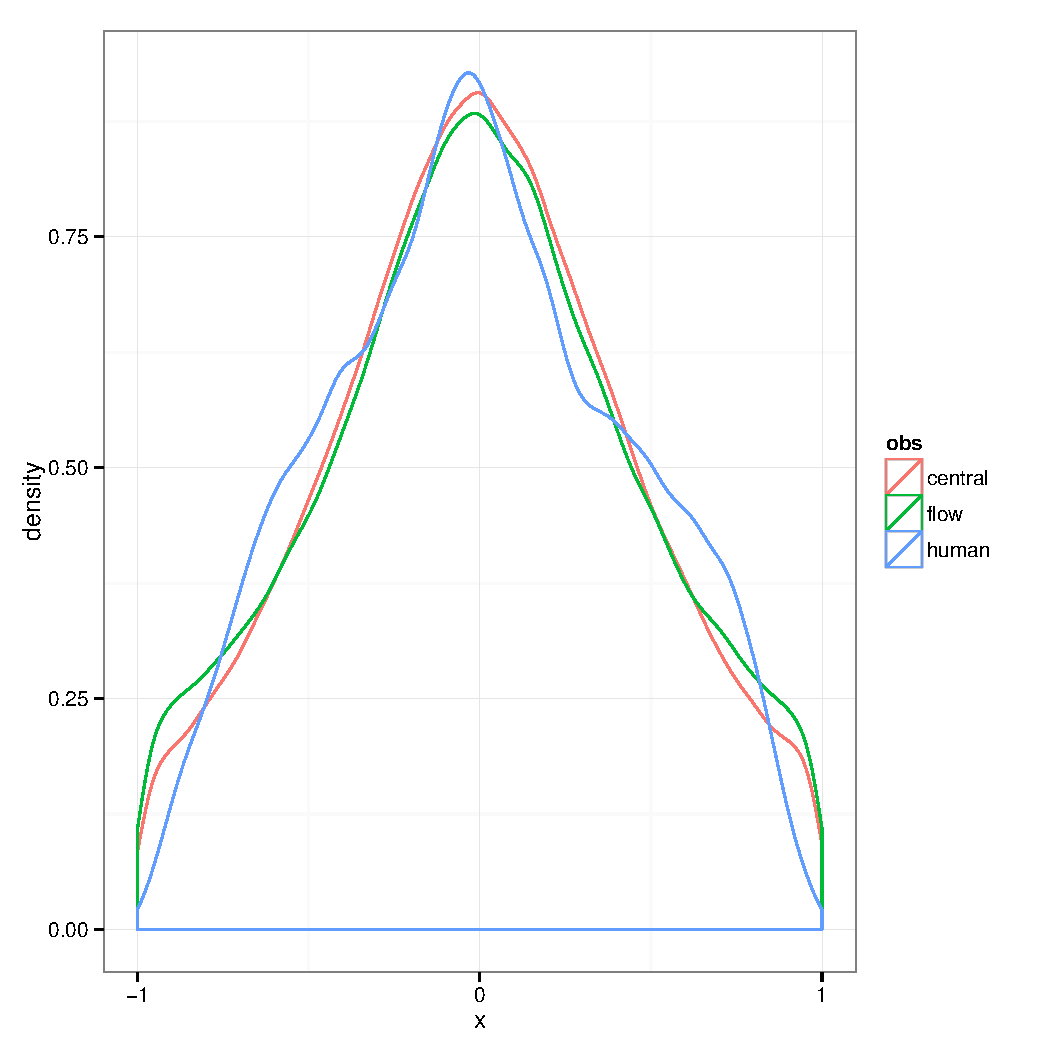
\includegraphics[width=3.8cm]{../scripts/coarse2fine/figs/xFixComparison}}
\subfigure{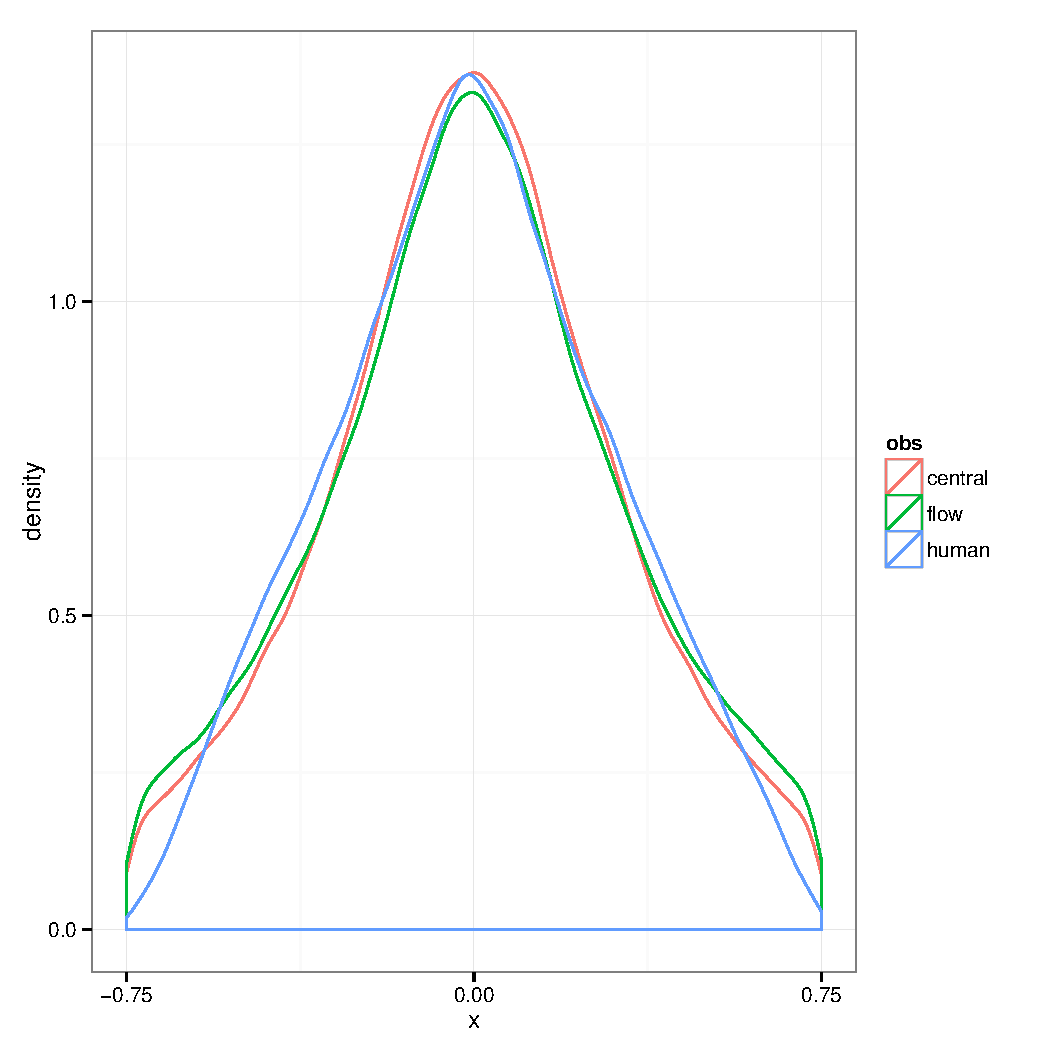
\includegraphics[width=3.8cm]{../scripts/coarse2fine/figs/yFixComparison}}
\subfigure{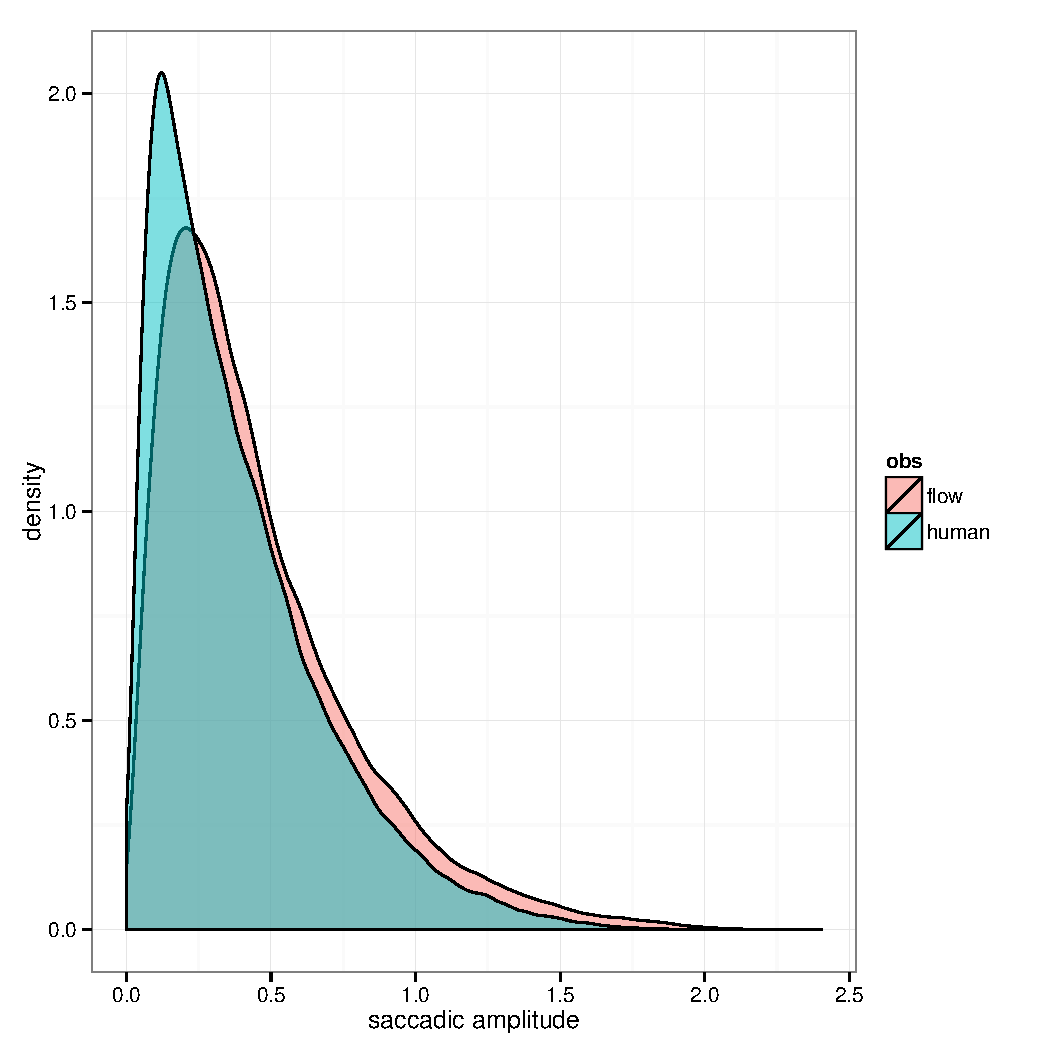
\includegraphics[width=3.8cm]{../scripts/coarse2fine/figs/ampSaccComparison}}
\subfigure{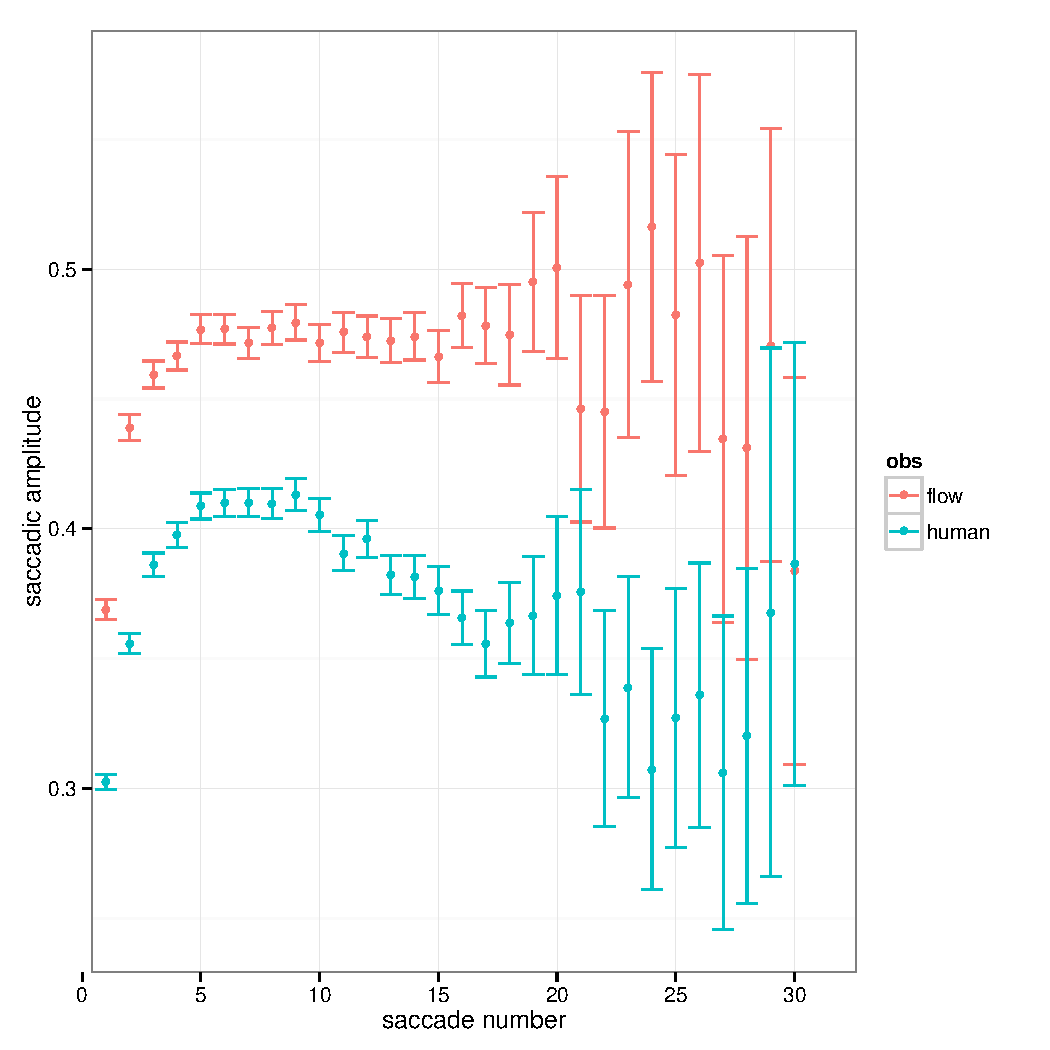
\includegraphics[width=3.8cm]{../scripts/coarse2fine/figs/saccAmpOverTimeFlow}}
\caption{\textit{blue}: human, \textit{red}: central bias, \textit{green}: saccadic flow. \textit{top row}: Comparison of $x$ and $y$ fixation positions between human fixations and synthetic points generated from the central bias and flow model. \textit{bottom row}: We can see that the flow model consistently makes saccades with a slightly larger amplitude than human observers. Distances are expressed relative to the width of the image.}
\label{fig:flowHumanComp}
\end{figure*}

\subsection{Discussion}

We have presented how biases such as saccadic flow and the central bias can be used in different ways. They can be used as a prior on the probability of making saccades to different regions of the image, allowing us to then more clearly visualise the image-dependant behaviour. These bias-weighted gaze landscapes can then be used in analysis as demonstrated in Section \ref{sec:reanalysisClarke2013}.

We can also use the bias distributions to generate data

